\section{On-demand evaluation for KBP}
\label{sec:application}
Applying the on-demand evaluation framework to a task requires us to answer three questions:
\begin{enumerate}
    \itemsep0pt
  \item What is the desired distribution over system predictions $p_i$?
  \item How do we label an instance $x$, i.e.\ check if $x \in \sY$?
  \item How do we sample from the unknown set of true instances $x \sim p_0$?
\end{enumerate}
In this section, we present practical implementations for knowledge base population.

\subsection{Sampling from system predictions}
% 1. what is the point of this distribution?
% - prevent over sampling instances.
%\ac{@PL:\@ I think that the role of $p_i$ is really very subtle, but very important. I hope the below paragraph highlights the paradigm shift in how one has to think about on-demand evaluation.}
Both the official TAC-KBP evaluation and the on-demand evaluation we propose use micro-averaged precision and recall as metrics. However, in the official evaluation, these metrics are computed over a fixed set of evaluation entities chosen by LDC annotators, resulting in two problems: (a) defining evaluation entities requires human intervention and (b) typically a large source of variability in evaluation scores comes from not having enough evaluation entities (see e.g.\ \citep{webber2010measurement}). In our methodology, we replace manually chosen evaluation entities by sampling entities from each system’s output according $p_i$. In effect, $p_i$ makes explicit the decision process of the annotator who chooses evaluation entities.

%\ac{@PL:\@ This paragraph goes into details, but I felt that it was useful to illustrate how we tailored a distribution to meet our evaluation goals.}
Identifying a reasonable distribution $p_i$ is an important implementation decision that depends on what one wishes to evaluate.
Our goal for the on-demand evaluation service we have implemented is to ensure that KBP systems are fairly evaluated on diverse subjects and predicates, while at the same time, ensuring that entities with multiple relations are represented to measure completeness of knowledge base entries.
As a result, we propose a distribution that is inversely proportional to the frequency of the subject and predicate and is proportional to the number of unique relations identified for an entity (to measure knowledge base completeness).
See \refapp{implementation} in the supplementary material for an analysis of this distribution and a study of other potential choices.

%Recall that a KBP system predicts a set of relation instances of the form (\entity{subject}, \relation{predicate}, \entity{object}, \textsc{provenance}).
%Simply choosing $p_i$ to be the uniform distribution over this set causes our evaluation metrics to be be dominated by a few common predicates (e.g.\ professional titles) or subject entities (e.g.\ ``United States of America'').
%Instead, we propose the following distribution which we reasonably approximates our goals:\footnote{
%See \refapp{implementation} for an analysis of this distribution and a study of other potential choices.} 
%\begin{align*}
%  p_i(x) &\eqdef \frac{\operatorname{\#uniq-relns}_i(x)}{\operatorname{\#pred-insts}_i(x) \operatorname{\#subj-insts}_i(x)},
%\end{align*}
%where $\operatorname{\#uniq-relns}_i(x)$ measures the number of unique relations (\entity{subject}, \relation{predicate}, \entity{object} triples) with the same \entity{subject} as $x$ in the system's output $X_i$, 
%$\operatorname{\#pred-insts}_i(x)$ measures the number of instances with the same \relation{predicate} as $x$ in $X_i$ and 
%$\operatorname{\#subj-insts}_i(x)$ measures the number of instances with the same \relation{subject} as $x$ in $X_i$.

%%The choice of distribution over this set determines how much we put weight on rare predicates and subject entities in our evaluation metric. % in our precision score. % PL: for recall 
%We therefore propose two instance distributions that evaluate precision and recall scores macro-averaged over predicates and subject entities, respectively:
%\begin{align*}
%  p_i^\text{(pred)}(x) &\eqdef \frac{1}{\operatorname{\#preds}(X_i)} \frac{1}{\operatorname{\#insts}(X_i, \relation{pred}(x))} \\
%  p_i^\text{(subj)}(x) &\eqdef \frac{1}{\operatorname{\#subjs}(X_i)} \frac{1}{\operatorname{\#insts}(X_i, \relation{subj}(x))}
%\end{align*}
%where $\operatorname{\#preds}$, $\operatorname{\#nsubjs}$ specifies the number of predicates, subject entities in $X_i$ respectively and $\operatorname{\#insts}$ the number of instances with the given predicate or subject entity.
%See \refapp{implementation} for more details.

\subsection{Labeling predicted instances}
We label predicted relation instances by presenting the instance's provenance to crowdworkers
  and asking them to identify if a relation holds between the identified subject and object mentions (\reffig{relation-interface}). 
  Crowdworkers are also asked to link the subject and object mentions to their canonical mentions within the document and to pages on Wikipedia, if possible, for entity linking.
On average, we find that crowdworkers are able to perform this task in about 20 seconds, corresponding to about \$0.05 per instance.
We requested 5 crowdworkers to annotate a small set of 200 relation instances from the 2015 TAC-KBP corpus 
and measured a substantial inter-annotator agreement with a Fleiss' kappa of 0.61 with 3 crowdworkers and 0.62 with 5. % \pl{why does it go up with more annotators?}.
%On manually inspection of these instances, we observed a precision of about 75\%.
%While this precision is slightly less than the 80\% obtained by annotators at LDC \citep{ellis2016overview}, we believe it could be easily improved with appropriate changes to the annotation interface.
Consequently, we take a majority vote over 3 workers in subsequent experiments.
%leading to a total cost of \$0.15 per relation instance.

%\pl{what does it mean to annotate a relation - get all the relation instances for that relation or just one?}.
\begin{figure*}
  \centering

  \begin{subfigure}{0.49\textwidth}
  \centering
    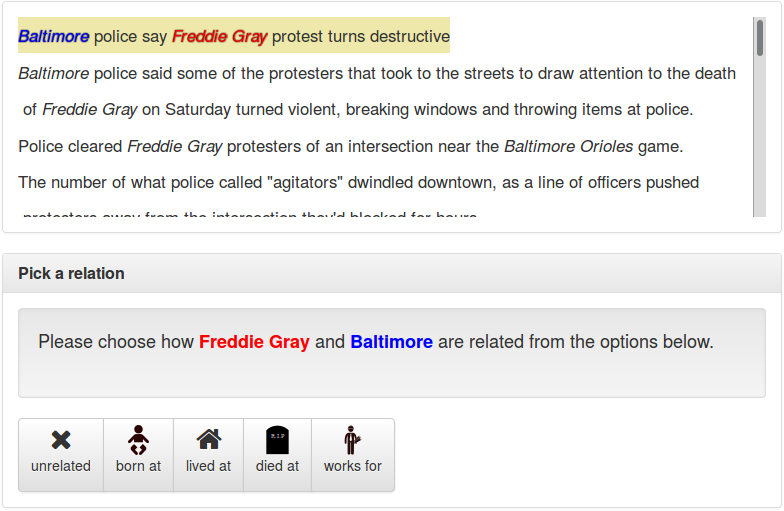
\includegraphics[width=\textwidth]{figures/interface/relation-interface}
    \caption{\label{fig:relation-interface}}
  \end{subfigure}
  \hfill
  \begin{subfigure}{0.49\textwidth}
  \centering
    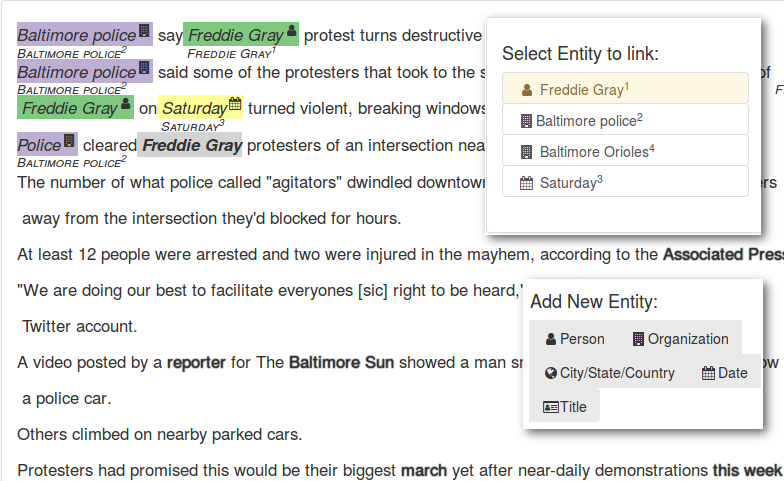
\includegraphics[width=\textwidth]{figures/interface/extraction-interface}
    \caption{\label{fig:entity-interface}}
  \end{subfigure} \\

  \begin{subfigure}{0.49\textwidth}
    \centering
    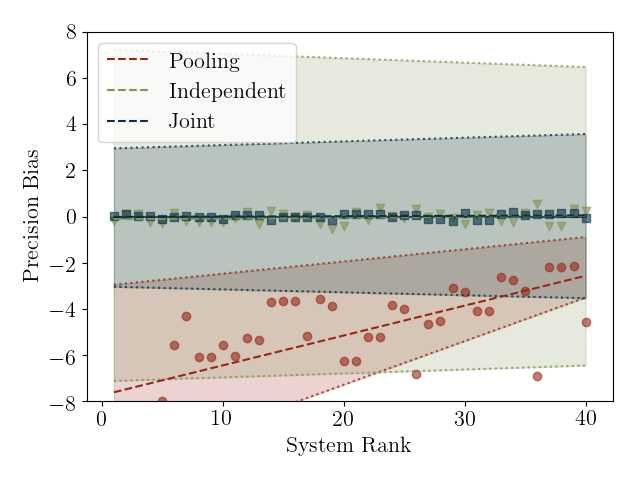
\includegraphics[width=\textwidth]{figures/simulation/simulation-p}
    \caption{}
  \end{subfigure}
  \hfill
  \begin{subfigure}{0.49\textwidth}
    \centering
    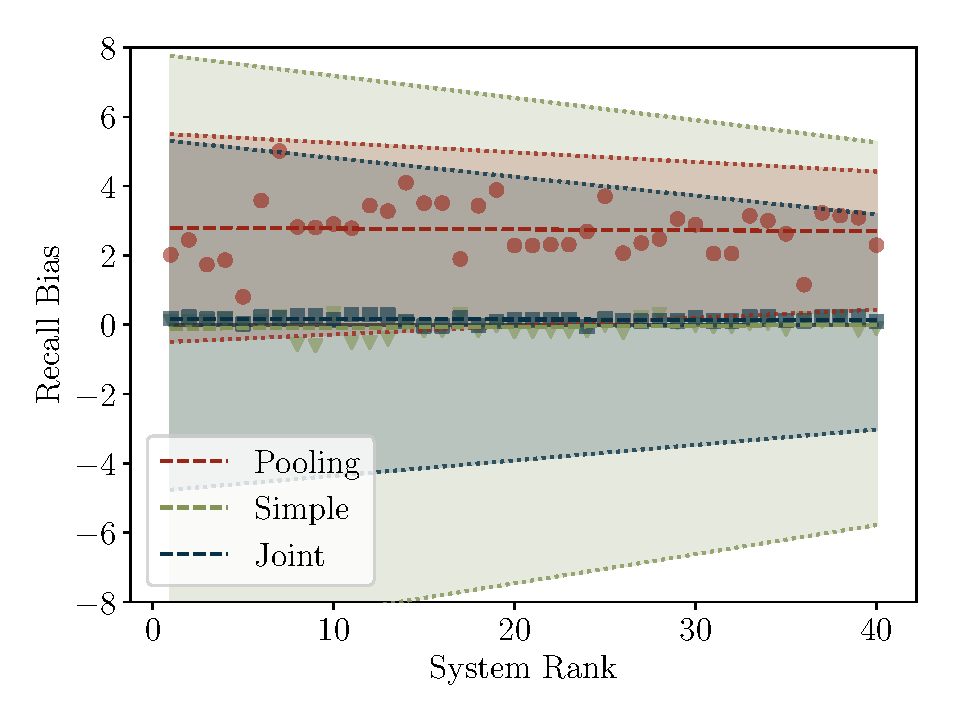
\includegraphics[width=\textwidth]{figures/simulation/simulation-r}
    \caption{}
  \end{subfigure} \\

  \begin{subfigure}{0.49\textwidth}
    \centering
    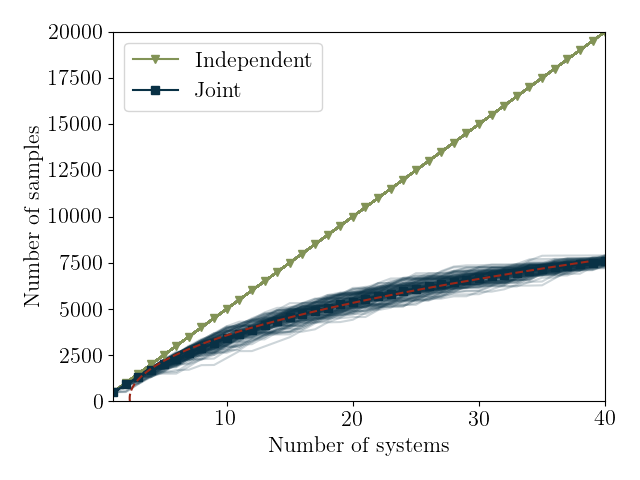
\includegraphics[width=\textwidth]{figures/simulation/simulation-n}
    \caption{}
  \end{subfigure}
  \hfill
  \begin{subfigure}{0.49\textwidth}
    \centering
    \begin{figure*}[th]
  \centering
  \begin{subfigure}[b]{0.45\textwidth}
  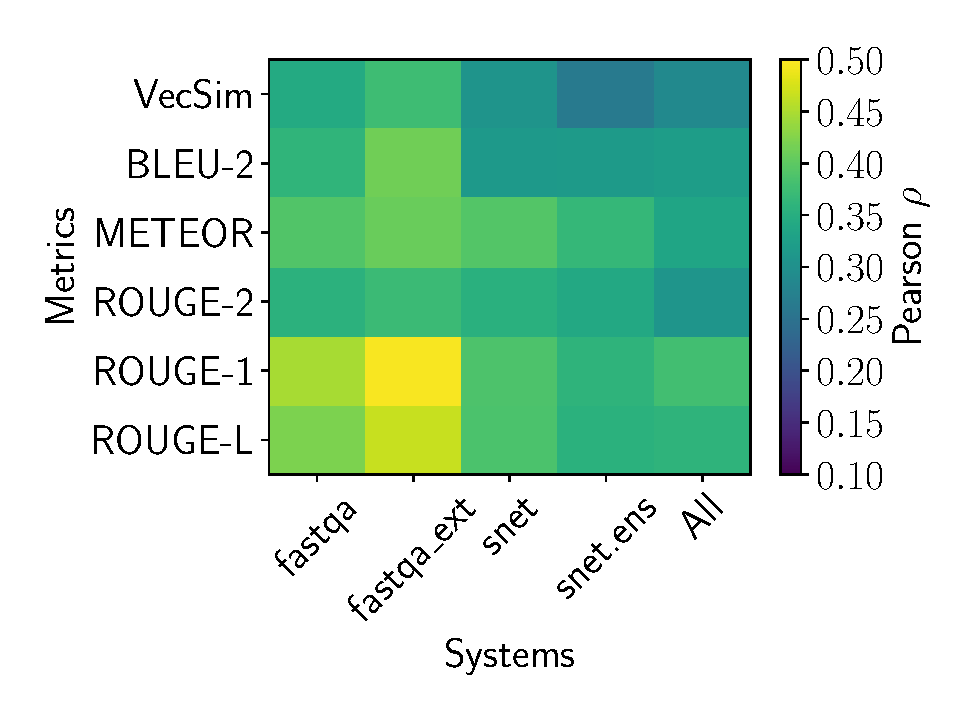
\includegraphics[width=\textwidth]{figures/msmarco_correlation}
  \caption{MS MARCO with the \texttt{AnyCorrect} prompt}
  \end{subfigure} \hfill
  \centering
  \begin{subfigure}[b]{0.45\textwidth}
  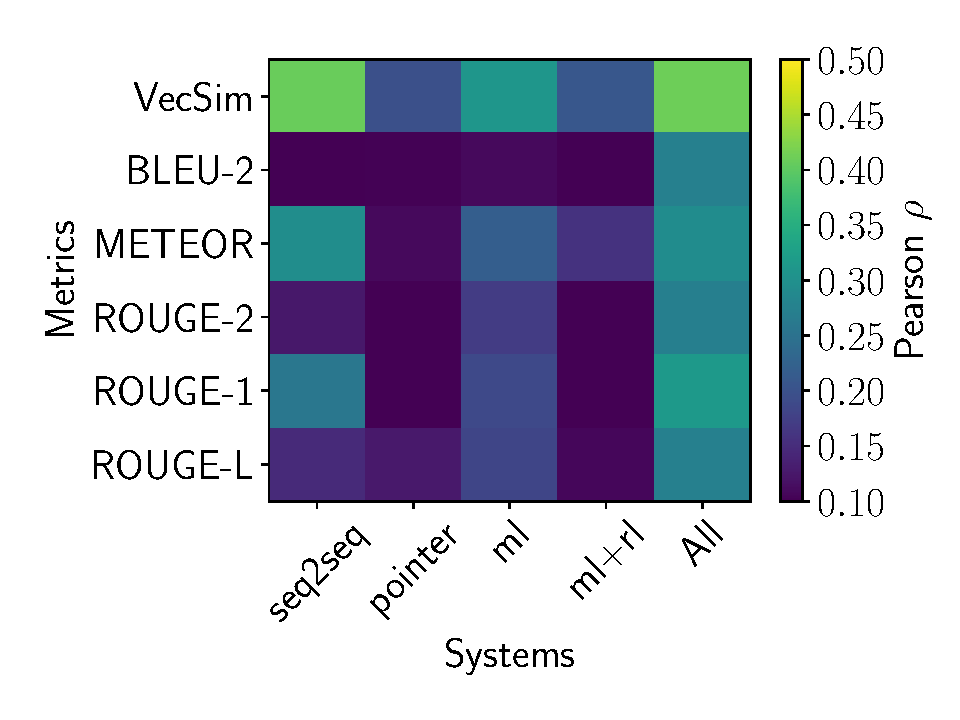
\includegraphics[width=\textwidth]{figures/lqual_correlation}
  \caption{CNN/Daily Mail with the \texttt{Edit} prompt}
  \end{subfigure}
  \caption{\label{fig:correlation} Correlations of different automatic metrics on the MS MARCO and CNN/Daily Mail tasks.
  Certain systems are more correlated with certain automatic metrics than others, but overall the correlation is low to moderate for most systems and metrics.
  }
\end{figure*}


\section{\label{sec:evaluation}Experimental results}

We are now ready to evaluate the performance of our control variates estimator proposed in \refsec{method} using the datasets presented in \refsec{tasks}.
Recall that our primary quantity of interest is \textit{data efficiency}, the ratio of the number of human judgments required to estimate the overall human evaluation score for the control variates estimator versus the sample mean.
We'll briefly review the automatic metrics used in our evaluation before analyzing the results.

%\begin{figure}[t]
%  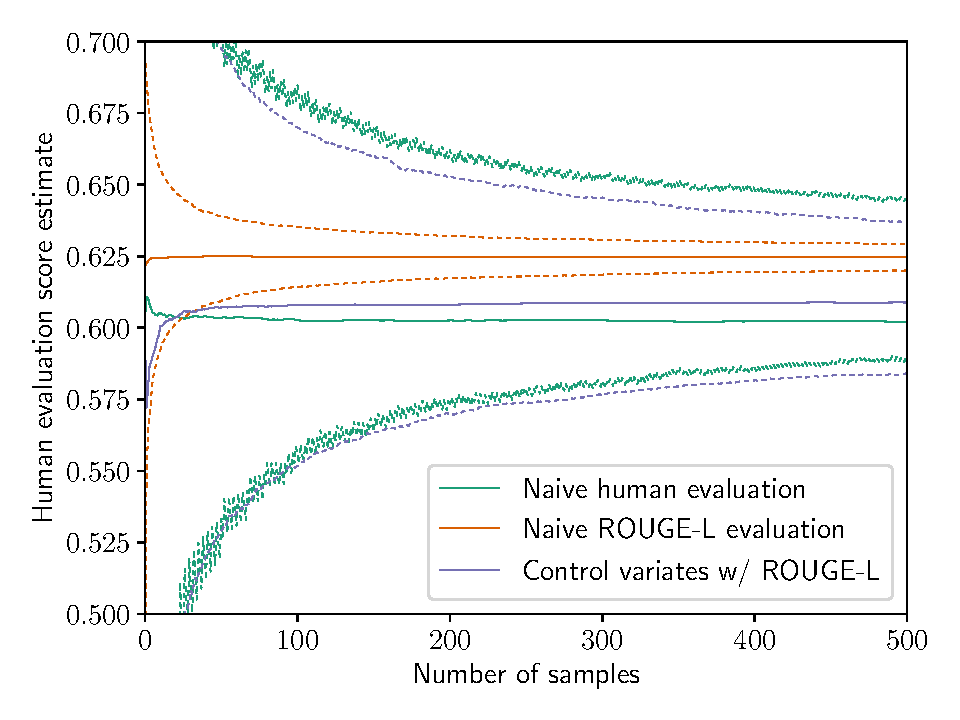
\includegraphics[width=\columnwidth]{figures/msmarco_full_trajectory}
%  \caption{\label{fig:bias-trajectory} A comparison of the human score estimates made by (a) naively sampling humans, (b) scaling and shifting the best automatic metric (ROUGE-L) and (c) incorporating the automatic metric into the control variates estimator proposed in this paper.
%  While (c) does not significantly reduce variance in its estimates, it is still an unbiased estimation of the human evaluation score, unlike (b).
%  The low confidence interval for the ROUGE-L scores are because they do not observe any annotator noise.
%  \ac{The curves are not exactly aligned because of a minor error in data for this plots. It will be fixed.}
%  }
%\end{figure}

% Evaluation
\paragraph{Automatic metrics.}
We consider the following frequently used automatic word-overlap based metrics in our work:
\textbf{BLEU}~\citep{papineni02bleu}, \textbf{ROUGE}~\citep{lin2004rouge} and \textbf{METEOR}~\citep{lavie2009meteor}.
Following \citet{novikova2017why} and \citet{liu2016evaluate}, we also compared a vector-based sentence-similarity using \texttt{sent2vec}~\citep{pagliardini2017unsupervised} to compare sentences (\textbf{VecSim}).
\reffig{correlation} shows how each of these metrics is correlated with human judgment for the systems being evaluated.
Unsurprisingly, the correlation varies considerably across systems, with token-based metrics correlating more strongly for systems that are more extractive in nature (\texttt{fastqa} and \texttt{fastqa\_ext}).

%\reffig{bias-trajectory} shows a trajectory estimates for human evaluation scores using the baseline of naive human evaluation versus those with the proposed control variates method.\footnote{%
%  All confidence intervals reported here are measured using 5,000 bootstrap samples generated by picking uniformly from the examples from the system output and then uniformly from the human annotations on that example.
%  }
%We also plot the estimate produced using an automatic metric, namely ROUGE-L after being scaled and shifted to match human evaluation scores at the system-level.
%Here, we see that while the control variates approach does not significantly reduce variance in estimates, it remains unbiased when using the model, unlike using the automatic metric.

%\begin{figure*}[t]
%  \centering
%  \begin{subfigure}[b]{0.45\textwidth}
%    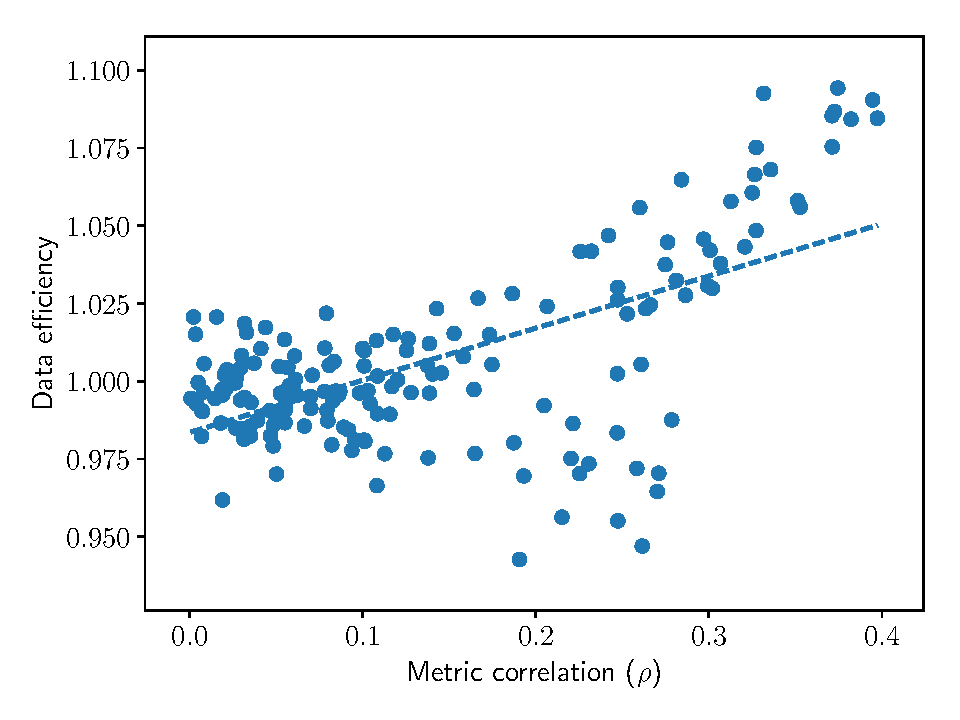
\includegraphics[width=\textwidth]{figures/de_vs_rho}
%  \end{subfigure} \hfill
%  \begin{subfigure}[b]{0.45\textwidth}
%    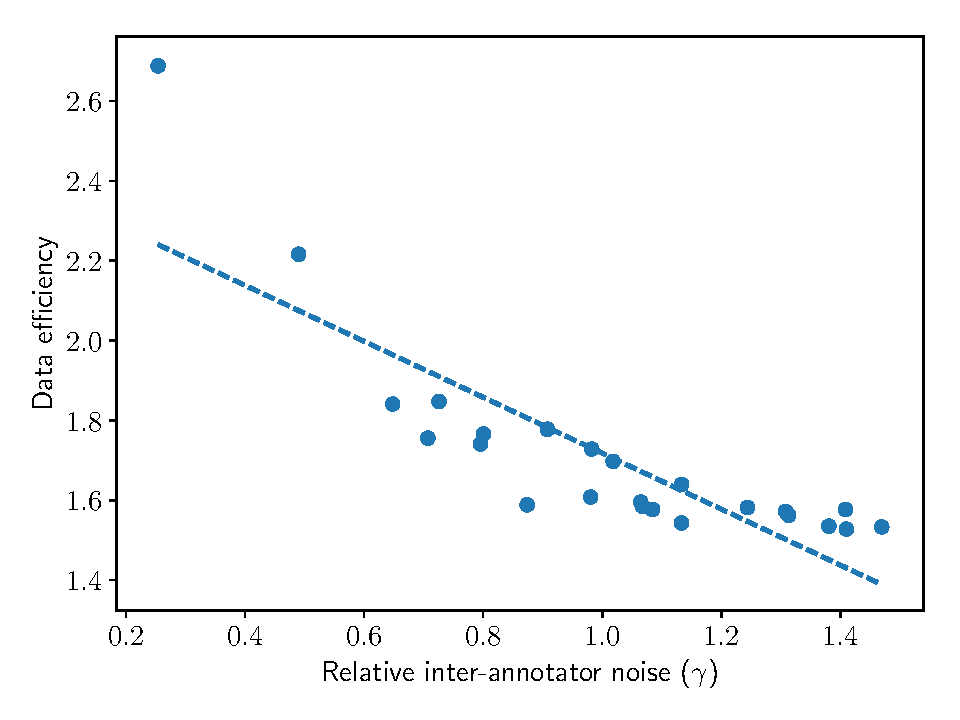
\includegraphics[width=\textwidth]{figures/de_vs_gamma}
%  \end{subfigure}
%  \caption{\label{fig:data-efficiency} A comparison of data efficiency possible across different systems and metrics. \ac{This figure seems like not very important so prefer ignoring.}}
%\end{figure*}

\begin{figure*}[th]
  \centering
  \begin{subfigure}[b]{0.32\textwidth}
  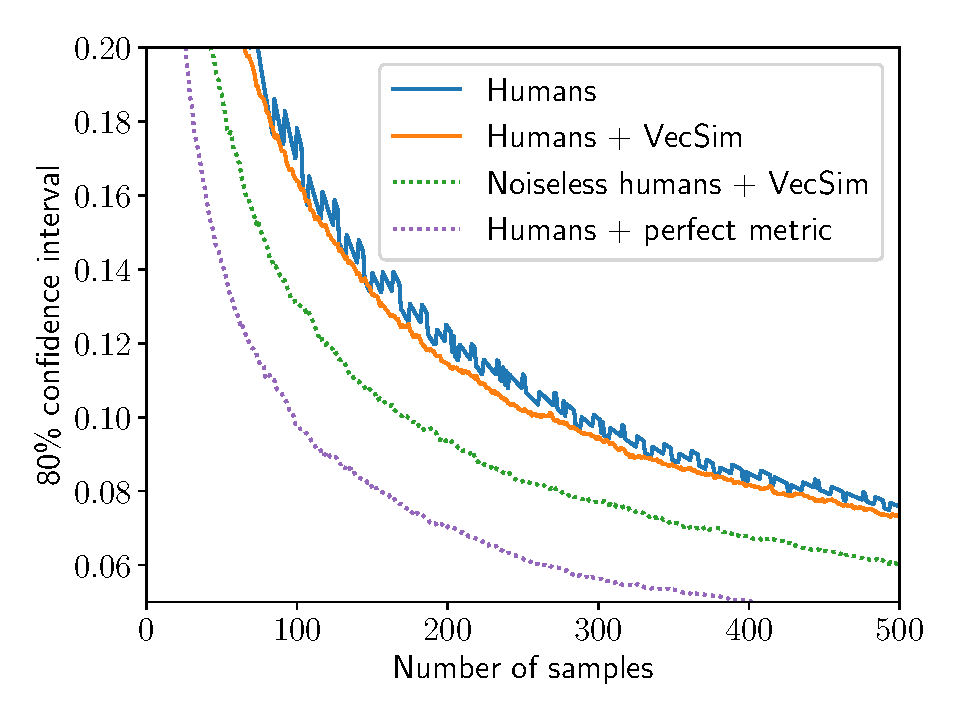
\includegraphics[width=\textwidth]{figures/lqual_trajectory_foil}
    \caption{\label{fig:trajectory-a}\texttt{seq2seq} on CNN/Daily Mail using the \texttt{Overall}}
  \end{subfigure} 
  \hfill
  \begin{subfigure}[b]{0.32\textwidth}
  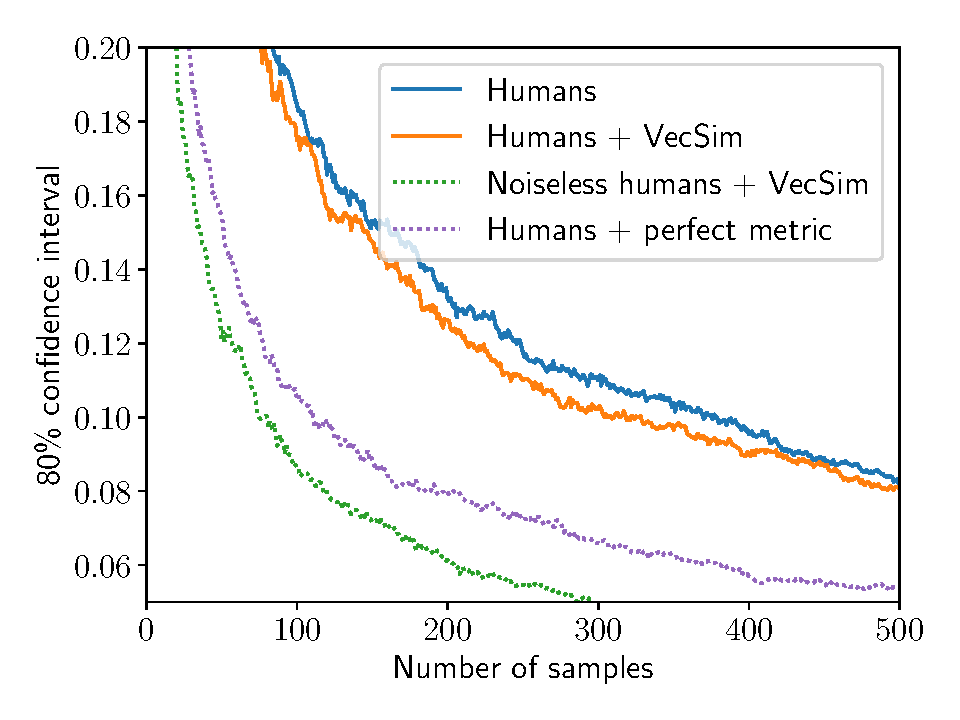
\includegraphics[width=\textwidth]{figures/lqual_trajectory}
  \caption{\label{fig:trajectory-b}\texttt{seq2seq} on CNN/Daily Mail using \texttt{Edit} }
  \end{subfigure}
  \hfill
  \begin{subfigure}[b]{0.32\textwidth}
  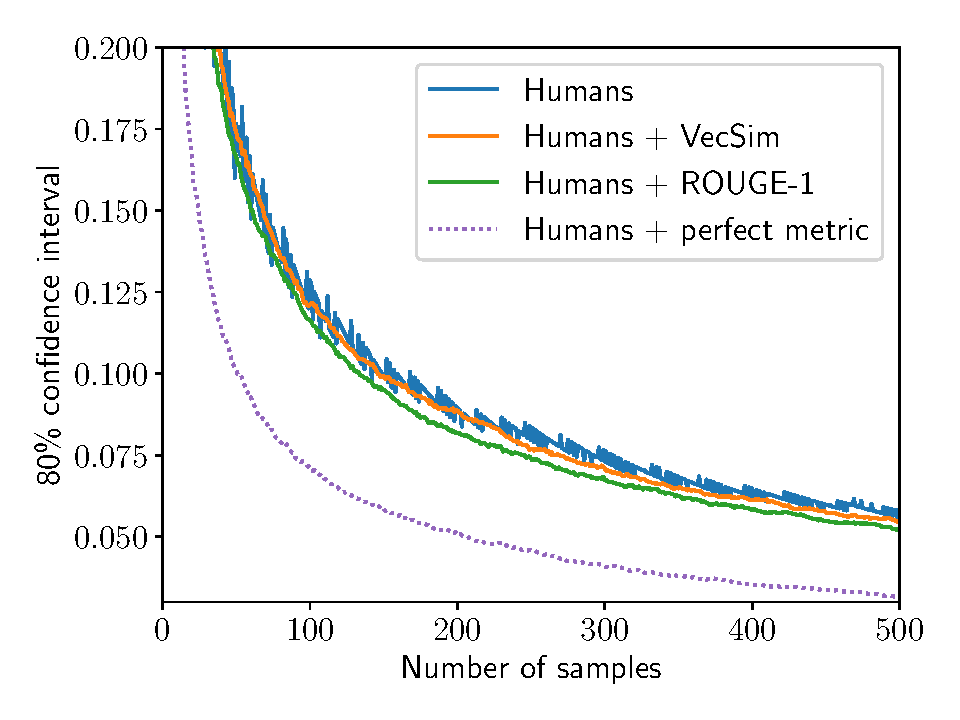
\includegraphics[width=\textwidth]{figures/msmarco_trajectory}
  \caption{\label{fig:trajectory-c}\texttt{fastqa\_ext} on MS MARCO using \texttt{AnyCorrect}}
  \end{subfigure}
  \caption{\label{fig:trajectory} 80\% bootstrap confidence interval length as a function of the number of human judgments used when evaluating the indicated systems on their respective datasets and prompts.
  (a) We see a modest reduction in variance (and hence cost) relative to human evaluation by using the VecSim automatic metric with the proposed control variates estimator to estimate \texttt{Overall} scores on the CNN/Daily Mail task; the data efficiency (DE) is $1.06$.
  (b) By improving the evaluation prompt to use \texttt{Edit}s instead, it is possible to further reduce variance relative to humans (DE is $1.15$).
  (c) Another way to reduce variance relative to humans is to improve the automatic metric evaluation; here using ROUGE-1 instead of VecSim improves the DE from $1.03$ to $1.16$.
  }
\end{figure*}

\paragraph{Results.}\footnote{%
  Extended results for other systems, metrics and prompts can be found at \url{https://bit.ly/price-of-debiasing/}.}
  
In \refsec{method} we proved that the control variates estimator is not only unbiased but also has the least variance among other unbiased estimators.
\reffig{trajectory} plots the width of the 80\% confidence interval, estimated using bootstrap, measured as a function of the number of samples collected for different tasks and prompts.
As expected, the control variates estimator reduces the width of the confidence interval. 
We measure data efficiency by the averaging of the ratio of squared confidence intervals between the human baseline and control variates estimates.
We observe that the data efficiency depends on the task, prompt and system, ranging from about 1.08 (a 7\% cost reduction) to 1.15 (a 13\% cost reduction) using current automatic metrics.

As we showed in \refsec{method}, further gains are fundamentally limited by the quality of the evaluation prompts and automatic metrics.
Figures~\ref{fig:trajectory-a} and~\ref{fig:trajectory-b} show how improving the quality of the evaluation prompt from a Likert-scale prompt for quality (\texttt{Overall}) to using post-editing (\texttt{Edit}) noticeably decreases variance and hence allows better automatic metrics to increase data efficiency.
Likewise, \reffig{trajectory-c} shows how using a better automatic metric (ROUGE-L instead of VecSim) also reduces variance.

%Note that even we were used ``a perfect metric'', i.e.\ one that had a correlation $\rho = 1$, we must collect at least a few human annotations to find out if the metric is indeed correct. \stm{I covered this case in the method section. Cut?}
%As a result, we might expect that annotator noise will still limit the data efficiency when using a perfect metric.
\reffig{trajectory} also shows the conjectured confidence intervals if we were able to eliminate noise in human judgments (noiseless humans) or have a automatic metric that correlated perfectly with average human judgment (perfect metric).
In particular, we use the mean of all (2--3) humans on each $z$ for the perfect $g(z)$ and use the mean of all humans on each $z$ for the ``noiseless'' $Y(z)$.
% AC: We want to say that the conjectured confidence intervals are an over-estimate.
%  We note that using the mean of the human responses for the perfect $g(z)$ introduces some correlation with human responses
%These probably yield optimistic \pl{maybe just remove this sentence, because we're already being optimistic; this is additional optimism, which might be confusing} data efficiencies because we don't have access to the true mean $f(z)$; further, the estimated perfect $g(z)$ we use is correlated with human judgments and hence ``corrects'' for their variance.

In both cases, we are able to significantly increase data efficiency (i.e.\ decrease estimator variance).
%but the data efficiency is capped based on the automatic metrics' correlation or the annotator noise respectively.
With zero annotator variance and using existing automatic metrics,
the data efficiency ranges from 1.42 to 1.69. With automatic metrics with perfect correlation and current variance of human judgments,
it ranges from 2.38 to 7.25.
%as shown in \reffig{data-efficiency}.
Thus, we conclude that it is important not only to improve our automatic metrics but also the evaluation prompts we use during human evaluation. 

    %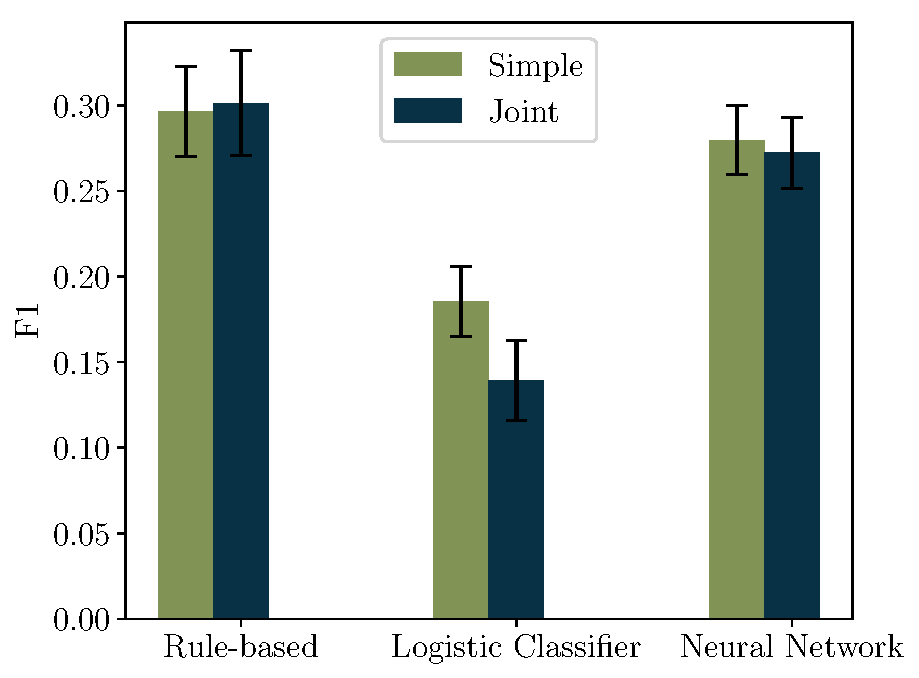
\includegraphics[width=\columnwidth]{figures/kbp2016/kbp2016_f1}
    \vfill
    \caption{\label{fig:evaluation-results}}
  \end{subfigure}

  \caption{\label{fig:simulation}
  \textbf{(a, b):} Interfaces for annotating relations and entities respectively.
  \textbf{(c, d):}
  A comparison of bias for the pooling, simple and joint estimators on the TAC KBP 2015 challenge.
  Each point in the figure is a mean of 500 repeated trials; dotted lines show the 90\% quartile.
  %The pooling based method uses between 5,000 and 6,000 labeled instances, while the sampling based methods use 
  %approximately 150 samples from each system.
  %Dashed trend lines indicate the mean bias of the estimation method: 
  %Unbiased estimates lie on the $y = x$ line.
  Both the simple and joint estimators are unbiased, and the joint estimator is able to significantly reduce variance.
  \textbf{(e):} 
  A comparison of the number of samples used to estimate scores under the fixed and adaptive sample selection scheme.
  %In the simulation, the top 40 systems were evaluated in randomized order to achieve a target variance equal to that obtained with 500 samples for a single system.
  Each faint line shows the number of samples used during a single trial, while solid lines show the mean over 100 trials.
  The dashed line shows a square-root relationship between the number of systems evaluated and the number of samples required.
  %\ac{Note: fitting with a cubic gives $x = 0.01 y^3 -0.1y^2 + 1.8 y - 1.1$ with $R=1.0$.}
  Thus joint estimation combined with adaptive sample selection can reduce the number of labeled annotations required by an order of magnitude.
  \textbf{(f):} 
Precision ($P$), recall ($R$) and \fone{} scores from a pilot run of our evaluation service for ensembles of a rule-based system (R), a logistic classifier (L) and a neural network classifier (N) run on the TAC KBP 2016 document corpus. 
  }
\end{figure*}

\subsection{Sampling true instances}
Sampling from the set of true instances $\sY$ is difficult because we can't even enumerate the elements of $\sY$.
As a proxy, we assume that relations are identically distributed across documents and have crowdworkers annotate a random subset of documents for relations using an interface we developed (\reffig{entity-interface}).
Crowdworkers begin by identifying every mention span in a document.
  For each mention, they are asked to identify its type, canonical mention within the document
  and associated Wikipedia page if possible.
They are then presented with a separate interface to label predicates between pairs of mentions within a sentence that were identified earlier.

We compare crowdsourced annotations against those of expert annotators using data from the TAC KBP 2015 EDL task on 10 randomly chosen documents.
We find that 3 crowdworkers together identify 92\% of the entity spans identified by expert annotators, while 7 crowdworkers together identify 96\%.
When using a token-level majority vote to identify entities, 3 crowdworkers identify about 78\% of the entity spans; this number does not change significantly with additional crowdworkers.
We also measure substantial token-level inter-annotator agreement using Fleiss' kappa for identifying typed mention spans ($\kappa = 0.83$), canonical mentions ($\kappa = 0.75$) and entity links ($\kappa = 0.75$) with just three workers.
Based on this analysis, we use token-level majority over 3 workers in subsequent experiments.
%We also manually labeled 200 relation instances that from the exhaustively annotated documents and observed a precision of about 75\%.
%While this precision is slightly less than the 80\% obtained by annotators at LDC \citep{ellis2016overview}, we believe it could be easily improved with appropriate changes to the annotation interface.

The entity annotation interface is far more involved and takes on average about 13 minutes per document, corresponding to about \$2.60 per document, while the relation annotation interface takes on average about \$2.25 per document.
Because documents vary significantly in length and complexity, we set rewards for each document based on the number of tokens (.75c per token) and mention pairs (5c per pair) respectively.
With 3 workers per document, we paid about \$15 per document on average.
Each document contained an average 9.2 relations, resulting in a cost of about \$1.61 per relation instance.
We note that this is about ten times as much as labeling a relation instance.

We defer details regarding how documents themselves should be weighted to capture diverse entities that span documents to \refapp{implementation}.
%We provide details regarding our sampling scheme and its distribution over entities in \refapp{implementation} of the supplementary material.
%When considering uniformly sampled documents, we found that a majority of the relations extracted correspond to very rare entities and result in very few entities with more than one relation (\reffig{entity-distribution}).
%In contrast, the TAC KBP query are almost evenly split between rare and semi-frequent entities.
%As a heuristic, we adopt the following two-stage sampling procedure:
%First, 20\% of our exhaustive document collection is sampled uniformly and annotated.
%We then uniformly sample the entities annotated to create a collection of ``evaluation entities''.
%Finally, we construct the remaining 80\% of our document collection by searching for documents that contain the evaluation entities according to an exact string match. This process results in far more entities of medium frequency.
